\documentclass[12pt,a4paper]{article}
\usepackage[portuguese]{babel}
\usepackage[colorlinks,allcolors=blue]{hyperref}
\usepackage[margin=1in]{geometry}
\usepackage[utf8]{inputenc}
\usepackage{amsmath}
\usepackage{graphicx}
\newcommand{\dpar}[1]{\left(#1\right)}
\newcommand{\un}[1]{\mathrm{#1}}

\DeclareMathOperator{\sen}{sen}
\DeclareMathOperator{\pr}{pr}

\title{Física Geral I: Lista de exercícios 1}

\author{Data de entrega: 11 de abril de 2018}

\date{}

\begin{document}
\maketitle
\begin{enumerate}
	\item (0,5 pontos) A densidade do ferro é $7274\,\un{kg}/\un{m}^3$. Expresse essa densidade em $\un{g}/\un{cm}^3$.
	\item (0,5 pontos) Uma pessoa anda $3\,\un{km}$ ao norte, logo $3\,\un{km}$ ao leste e finalmente $1\,\un{km}$ ao sul. Determine a distância entre o ponto de partida e o ponto de chegada.
	\item (0,5 pontos) Se $\vec A=\hat i-2\hat j+3\hat k$ e $\vec B=2\hat i+5\hat j-4\hat k$. Determine o módulo dos vetores $\vec A+\vec B$ e $\vec A-\vec B$.
	\item (0,5 pontos) Sejam os vetores $\vec A=3\hat i-4\hat j-2\hat k$ e $\vec B=5\hat i+3\hat j$. Determine o ângulo formado entre esses vetores. 
	\item (0,5 pontos) Se $\vec A=\hat i+5\hat j-\hat k$ e $\vec B=2\hat i-3\hat j+\hat k$. Encontre um vetor $\vec C$ que seja perpendicular a $\vec A$ e a $\vec B$. 
	\item (0,5 pontos) Usando o fato de que $|\vec A|^2=\vec A\cdot\vec A$, demonstre a chamada \textbf{lei de cossenos}:
	$$|\vec A-\vec B|^2=|\vec A|^2+|\vec B|^2-2|\vec A||\vec B|\cos\theta\,,$$
	onde $\theta$ é o ângulo formado entre $\vec A$ e $\vec B$.
	\item (0,5 pontos) Dê um exemplo de três vetores $\vec A, \vec B$ e $\vec C$ tais que
	$$\vec A\times (\vec B\times \vec C)\ne (\vec A\times \vec B)\times\vec C\,.$$
	Dica: Analise produtos vetoriais envolvendo os vetores unitários $\hat i,\hat j$ e $\hat k$.
	\item (0,5 pontos) Sejam os vetores $\vec A=\hat i+\hat j$, $\vec B=\hat j+\hat k$ e $\hat C=\hat k+\hat i$. Calcule $\vec A\times (\vec B\times\vec C)$ e $(\vec A\cdot\vec C)\vec B-(\vec A\cdot\vec B)\vec C$.
	\item (0,5 pontos) Sem fazer cálculos, justifique que $\vec A\cdot (\vec B\times\vec C)=0$ quando $\vec B=c\vec A$, com $c\ne 0$.
	\item (0,5 pontos) A posição de um caminhão em cada instante de tempo está dada pela equação $x(t)=(0,5 \,\un{m}/\un{s}^3)t^3+(1\,\un{m}/\un{s}^2)t^2+5\,\un{m}$. Determine a velocidade média do caminhão entre os instantes $t=1\,\un s$ e $t=2\,\un s$. Determine também a velocidade instantânea do caminhão no instante $t=2\,\un s$.
	\item (1 ponto) Considere os vetores $\vec A, \vec B$ e $\vec C$ dados na figura~\ref{fig}. Se $|\vec A|=6$, $|\vec B|=2\sqrt{2}$ e $|\vec C|=4$, encontre o módulo do vetor $\vec R=\vec A+\vec B+\vec C$ e o ângulo que esse vetor faz com o eixo $x$ positivo.
	\begin{figure}
		\centering
		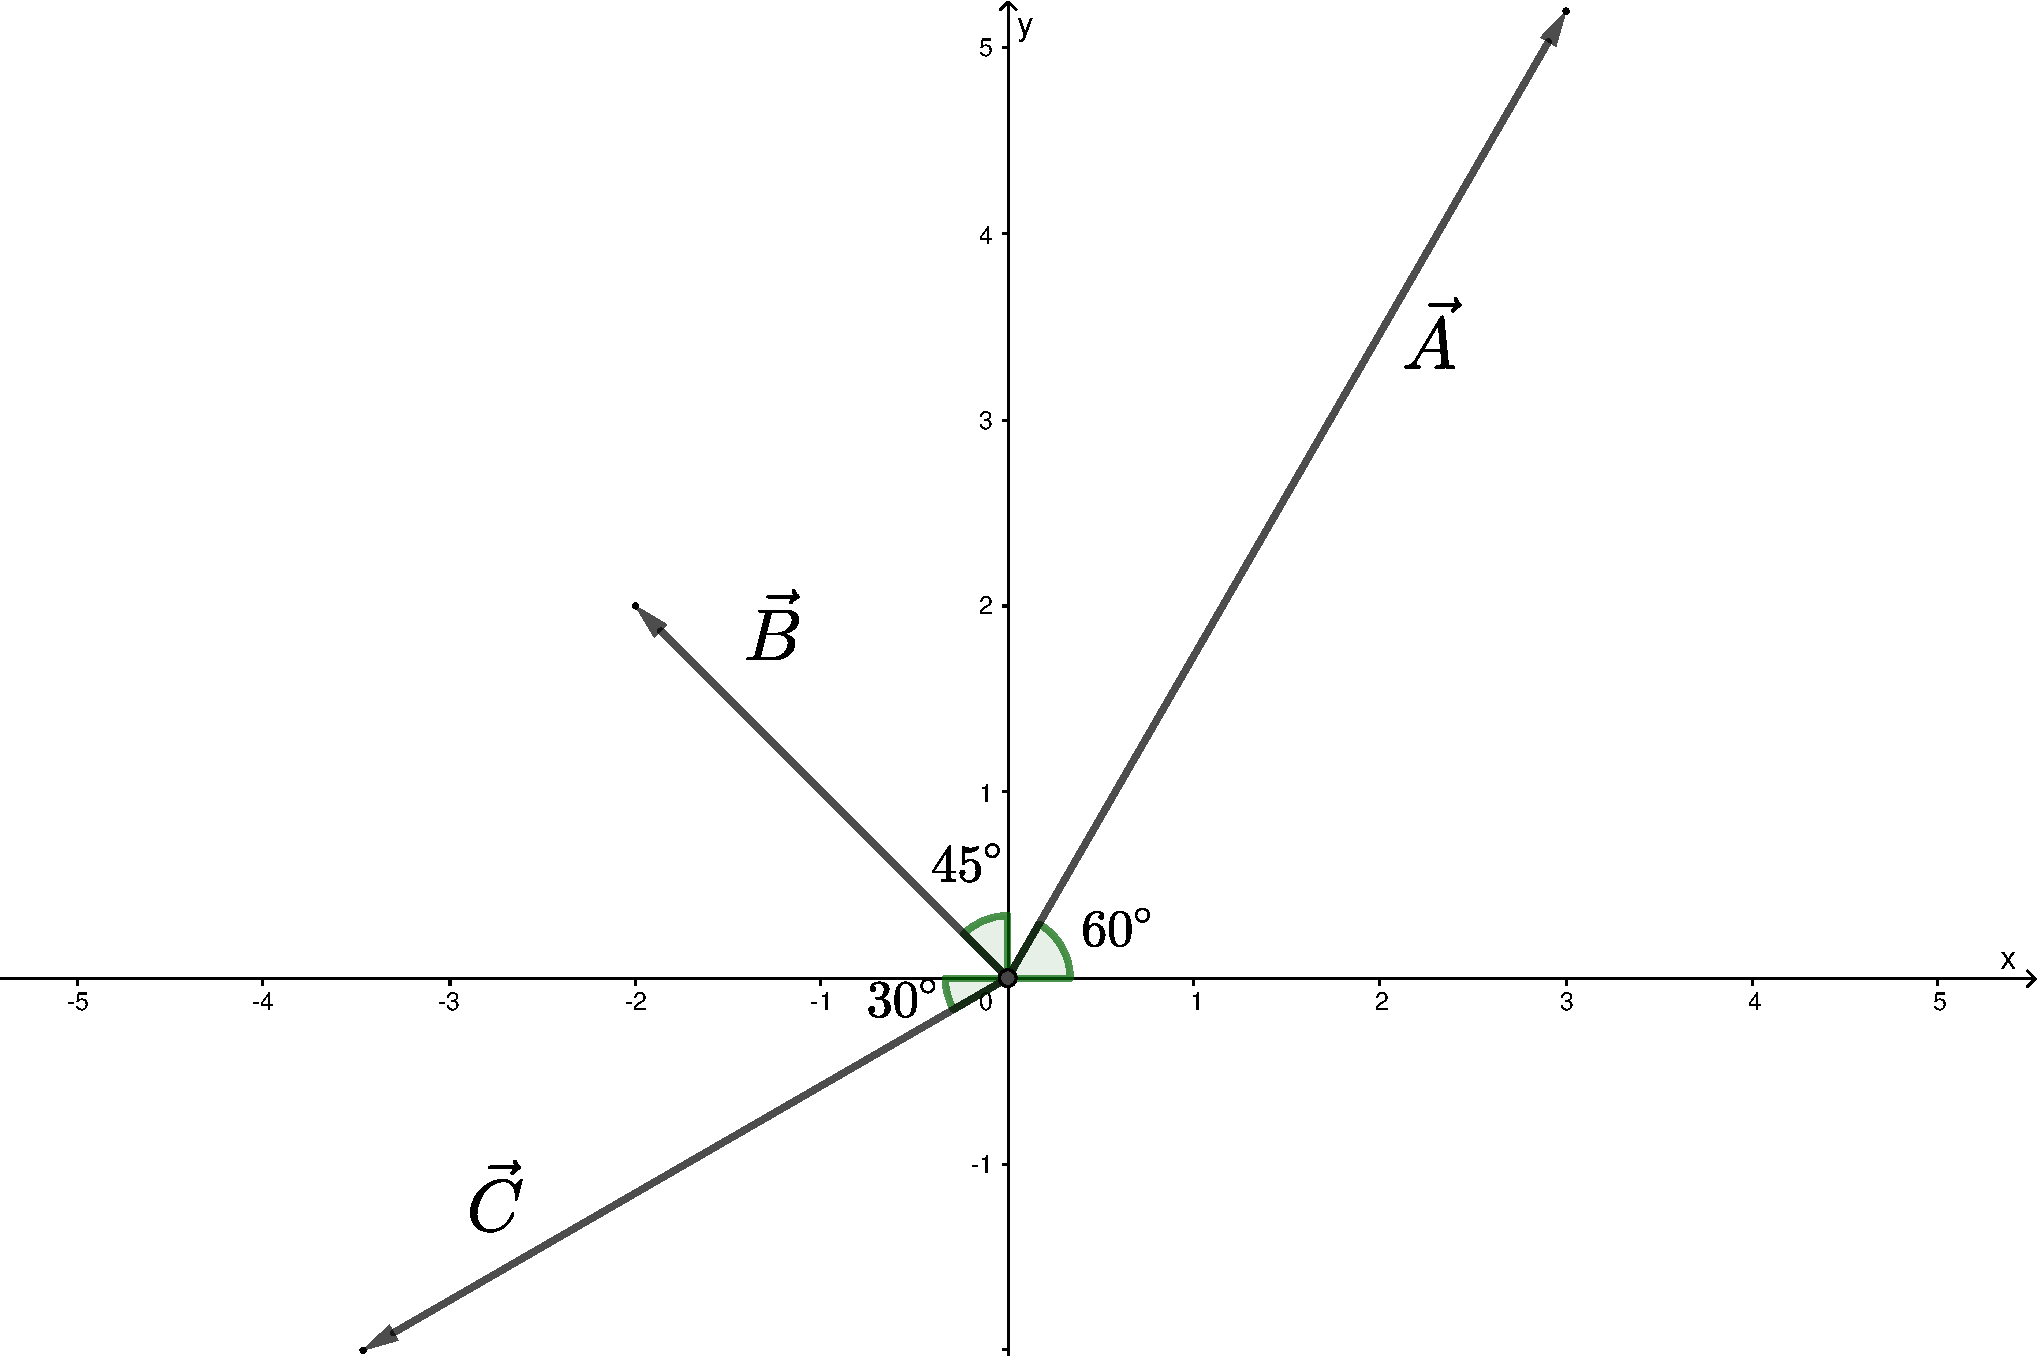
\includegraphics[width=0.9\textwidth,keepaspectratio]{questao11}
		\caption{Questões 11 e 12.}
		\label{fig}
	\end{figure}
	\item (1 ponto) Calcule o produto vetorial $\vec A\times\vec B$ usando as definições dos vetores $\vec A$ e $\vec B$ dadas na questão 11. Use o resultado para encontrar $\sen 75^\circ$ sem o uso de calculadora. Mostre que vale a relação $\sen 75^\circ=\sen 30^\circ\cos 45^\circ+\cos 30^\circ\sen 45^\circ$.
	\item (1 ponto) Dado um vetor não nulo $\vec A$, definimos a \textbf{projeção} de um vetor $\vec B$ sobre $\vec A$ como sendo o vetor
	$$\vec P=\dpar{\frac{\vec A\cdot \vec B}{|\vec A|^2}}\vec A\,.$$
	Definindo o vetor $\vec C=\vec B-\vec P$, mostre que $\vec C\cdot\vec A=0$ e que $|\vec B|^2=|\vec C|^2+|\vec P|^2$.
	\item (1 ponto) Usando componentes, verifique que $\vec A\cdot(\vec B\times\vec C)=\vec B\cdot(\vec C\times \vec A)$ para quaisquer vetores $\vec A, \vec B$ e $\vec C$.
	\item (1 ponto) Um automóvel se move em linha reta de tal forma que sua posição é dada pela equação $x(t)=10\,\un{m}+(24\,\un{m}/\un{s})t-(18\,\un{m}/\un{s^2})t^2$. Responda as seguintes questões:
	\begin{enumerate}
		\item Qual é a posição inicial do automóvel ($t=0\,\un{s}$).
		\item O automóvel volta a passar por esse ponto? Em qual instante de tempo isso acontece?
		\item Em algum instante de tempo a posição do automóvel é $16\,\un{m}$? Res\-pon\-da a mesma pergunta para as posições $22\,\un{m}$ e $0\,\un{m}$.
		\item Descreva qualitativamente (em palavras) o movimento do automóvel.
	\end{enumerate}
\end{enumerate}
\end{document}